\documentclass[12pt]{scrartcl}
\usepackage{config}
\usepackage{minted}

%\newcommand\mrh{\color{white}\bfseries}
\newcommand\mrc[1]{\begin{tabular}{@{}l@{}} #1 \end{tabular}}
\setlength\arrayrulewidth{0.8pt}

\usemintedstyle{pastie}

\begin{document}
    \hh{Arbol-stían}
    
    
    \vspace{10pt}

    
    \hh{Problema}
    
        Te es dado un entero $N$ y $N - 1$ aristas bidireccionales. Estas aristas conectan $N$ vértices de tal forma que exista un camino entre cualesquiera dos vértices (es decir, forman un árbol). Además, cada vértice tiene un peso. Para cada camino, definimos su peso como el producto de la cantidad de aristas en él, y el {\bfseries máximo común divisor} de cada uno de los pesos de los vértices en el camino en el camino. Determina el camino simple (que no repite aristas) con peso máximo.
    
    \hh{Detalles de Implementación}

        Debes implementar la función $Arbol-stian()$. Esta función recibe un entero $N$, 2 vectores $u, v$ con $N - 1$ elementos, y un vector $w$, con $N$ elementos. Para cada $0 \le i \le N - 2$, $u[i]$ y $v[i]$ son los vértices que se conectan con la arista $i$. para cada $0 \le i \le N - 1$, $w[i]$ es el peso del vértice $i$. Esta función debe regresar un entero, el peso máximo en camino del árbol.
        La función se vería así:

\begin{minted}{c++}
#include <bits/stdc++.h>
using namespace std;

long long int Arbol-stian(int N, vector<int> u, vector<int> v, vector<int> w) {
    // Implementa esta función.
}
    
\end{minted}

    El evaluador llamará la función una sola vez por caso de prueba.

    \hh{Ejemplos}
    
        {\itshape Ejemplo 1:}
        \begin{itemize}
            \item El evaluador llama la función $$Arbol-stian(6, \{0, 0, 0, 2, 3\}, \{1, 2, 3, 4, 5\}, \{8, 2, 2, 4, 4, 8\})$$ el árbol en este ejemplo es el siguiente:
            \begin{center}
                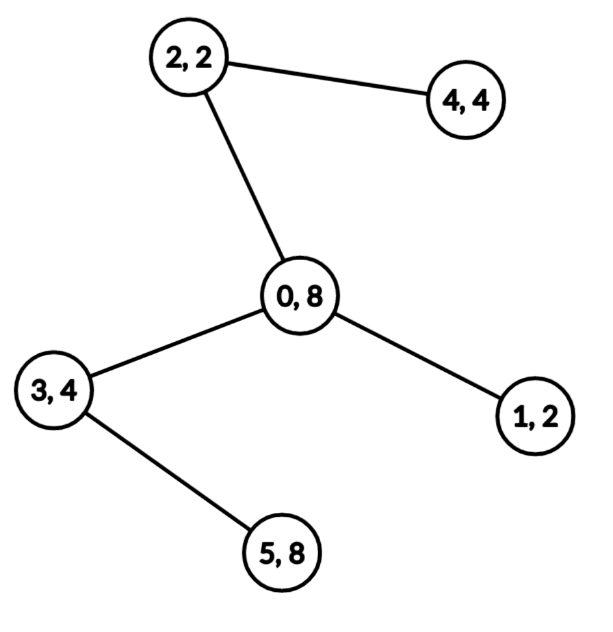
\includegraphics[scale=0.25]{ej1.png}
            \end{center}
            \item Los caminos posibles y sus pesos en este árbol son:
            \begin{center}
                \begin{tabular}{|c||c|c|c|c|c|c|}
                    \hline
                     $dist(a, b)$ & 0 & 1 & 2 & 3 & 4 & 5 \\
                     \hline
                     \hline
                     0 & 0 & 2 & 2 & 4 & 4 & 8 \\
                     \hline
                     1 & 2 & 0 & 4 & 4 & 6 & 6 \\
                     \hline
                     2 & 2 & 4 & 0 & 4 & 2 & 6 \\
                     \hline
                     3 & 4 & 4 & 4 & 0 & 6 & 4 \\
                     \hline
                     4 & 4 & 6 & 2 & 6 & 0 & 8 \\
                     \hline
                     5 & 8 & 6 & 6 & 4 & 8 & 0 \\ 
                     \hline
                \end{tabular}
            \end{center}
            \item La respuesta correcta es $8$.
        \end{itemize}

        {\itshape Ejemplo 2:}
        \begin{itemize}
            \item El evaluador llama la función $$Arbol-stian(9, \{0, 1, 2, 3, 4, 5, 6, 7\}, \{1, 2, 3, 4, 5, 6, 7, 8\}, \{3, 3, 15, 10, 14, 7, 21, 6, 2\})$$ el árbol en este ejemplo es el siguiente:
            \begin{center}
                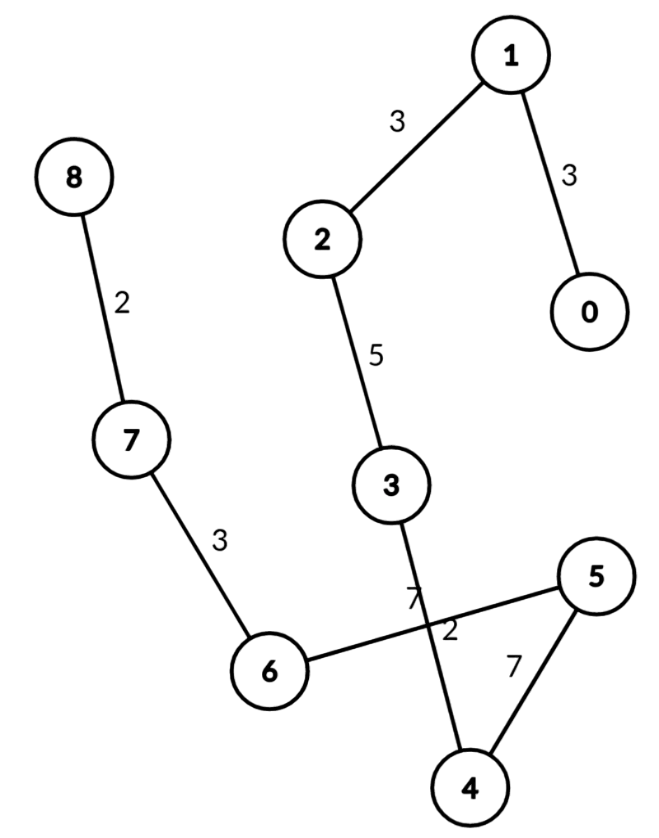
\includegraphics[scale=0.25]{ej2.png}
            \end{center}
            \item La respuesta correcta es $14$.
        \end{itemize}
        

    \hh{Consideraciones}
        \begin{itemize}
            \item $1 \le N \le 2\times10^5$.
            \item Los vectores $u$ y $v$ tendrán exactamente $N - 1$ elementos.
            \item El vector $w$ tendrá exactamente $N$ elementos.
            \item Para cada $0 \le i \le N - 2$, se cumple que $1 \le u[i] \neq v[i] \le N$. 
            \item Para cada $0 \le i \le N - 1$, se cumple que $0 \le w[i] \le 10^6$.
            \item Se garantiza que el grafo formado por las aristas es un árbol.
        \end{itemize}
    
    \hh{Subtareas}


    \begin{itemize}
        \item (3 puntos) $N \le 2000$.
        \item (9 puntos) Para todo $0 \le i \le N - 1$, se cumple que $w[i] \le 1$.
        \item (11 puntos) Para todo $0 \le i \le N - 2$, se cumple que $mcd(w[u[i]], w[v[i]])$ es un número primo.
        \item (22 puntos) Para todo $0 \le i \le N - 1$, se cumple que $w[i]$ es una potencia de 2.
        \item (22 puntos) Para todo $0 \le i \le N - 2$, se cumple que $u[i] = i + 1, v[i] = i + 2$.
        \item (33 puntos) Sin restricciones adicionales.
    \end{itemize}
\end{document}
